% !TEX encoding = UTF-8
%Koma article
\documentclass[fontsize=12pt,paper=letter,twoside]{scrartcl}
\usepackage{float}
\usepackage{listings}
\usepackage{color}
\definecolor{lightgray}{rgb}{.9,.9,.9}
\definecolor{darkgray}{rgb}{.4,.4,.4}
\definecolor{purple}{rgb}{0.65, 0.12, 0.82}

\lstdefinelanguage{JavaScript}{
  keywords={typeof, new, true, false, catch, function, return, null, catch, switch, var, if, in, while, do, else, case, break},
  keywordstyle=\color{blue}\bfseries,
  ndkeywords={class, export, boolean, throw, implements, import, this},
  ndkeywordstyle=\color{darkgray}\bfseries,
  identifierstyle=\color{black},
  sensitive=false,
  comment=[l]{//},
  morecomment=[s]{/*}{*/},
  commentstyle=\color{purple}\ttfamily,
  stringstyle=\color{red}\ttfamily,
  morestring=[b]',
  morestring=[b]"
}

\lstset{
   language=JavaScript,
   backgroundcolor=\color{lightgray},
   extendedchars=true,
   basicstyle=\footnotesize\ttfamily,
   showstringspaces=false,
   showspaces=false,
   numbers=left,
   numberstyle=\footnotesize,
   numbersep=9pt,
   tabsize=2,
   breaklines=true,
   showtabs=false,
   captionpos=b
}

%Standard Pre-amble
\usepackage[top=4cm,bottom=4cm,left=3cm,right=3cm,asymmetric]{geometry}
%\geometry{landscape}                % Activate for for rotated page geometry
%\usepackage[parfill]{parskip}    % Begin paragraphs with an empty line rather than an indent
\usepackage[table,xcdraw]{xcolor}
\usepackage{graphicx}

\usepackage{amsmath}
\usepackage{amssymb}
\usepackage{epstopdf}
\DeclareGraphicsRule{.tif}{png}{.png}{`convert #1 `dirname #1`/`basename #1 .tif`.png}
% Listings needs package courier
\usepackage{listings} % Needs 
\usepackage{courier}

\usepackage[framemethod=TikZ]{mdframed}
\usepackage{url}

\usepackage{sty/bsymb} %% Event-B symbols
\usepackage{sty/eventB} %% REQ and ENV
\usepackage{sty/calculation}

%Maths
\usepackage{amssymb,amsmath}
\def\Fl{\mathbb{F}}
\def\Rl{\mathbb{R}}
\def\Nl{\mathbb{N}}
\def\Bl{\mathbb{B}}
\def\St{\mathbb{S}}
\newcommand{\ovr}{\upharpoonright}
\newcommand{\var}[1]{\textit{#1}}
%Useful definitions
\newcommand{\mv}[1]{\textit{m\_#1}}
\newcommand{\cv}[1]{\textit{c\_#1}}
\newcommand{\degree}[1]{^{\circ}\mathrm{#1}}
%\newcommand{\comment}[1]{{\footnotesize \quad\texttt{--}\textrm{#1}}}
\newcommand{\im}[1]{i\texttt{-\!#1}}

\usepackage[headsepline]{scrpage2}
\pagestyle{scrheadings}
\ihead[]{\small EECS4312 Report1}
\ohead[]{\small \thepage}
\cfoot[]{}
\ofoot[]{}


%%%%PVS environment%%%%%%%%%%%%%%%%%%%
\lstnewenvironment{pvs}[1][]
    {\lstset{#1,captionpos=b,language=pvs,
    mathescape=true,
    basicstyle=\small\ttfamily,
    numbers=none,
    frame=single,
    % numberstyle=\tiny\color{gray},
    % backgroundcolor=\color{lightgray},
    firstnumber=auto
    }}
    {}
 %%%%%%%%%%%%%%%%%%%%%%%%%%%%%%%%
 
%%%%Verbatim environment%%%%%%%%%%%%%%%%%%%
\lstnewenvironment{code}[1][]
    {\lstset{#1,captionpos=b,
    mathescape=true,
    basicstyle=\small\ttfamily,
    numbers=none,
    frame=single,
    % numberstyle=\tiny\color{gray},
    % backgroundcolor=\color{lightgray},
    firstnumber=auto
    }}
    {}

% \newenvironment{boxed}[1]
%    {\begin{center}
%    #1\\[1ex]
%    \begin{tabular}{|p{0.9\textwidth}|}
%    \hline\\
%    }
%    { 
%    \\\\\hline
%    \end{tabular} 
%    \end{center}
%    }
 %%%%%%%%%%%%%%%%%%%%%%%%%%%%%%%%
 
 %Text in a box
\newenvironment{textbox}
    {\begin{center}
    \begin{tabular}{|p{0.9\textwidth}|}
    \hline\\
    }
    { 
    \\\\\hline
    \end{tabular} 
    \end{center}
    }

\usepackage{hyperref}

%Highlight \hl{}
\usepackage{soul}

\usepackage{enumitem}
\newlist{mylist}{itemize}{1}
\setlist[mylist]{label=\textbullet,leftmargin=1cm,nosep}

\usepackage{multirow}

% Reduce space between figure and caption
%\usepackage{caption}
%\captionsetup[table]{font=small,skip=0pt}     %% Adjust here
%or equivalently 
\usepackage[font=small,skip=4pt]{caption}
%Useful definitions
%\newcommand{\mv}[1]{\textit{m\_#1}}
%\newcommand{\cv}[1]{\textit{c\_#1}}
%\newcommand{\degree}[1]{^{\circ}\mathrm{#1}}
%\newcommand{\comment}[1]{{\footnotesize \quad\texttt{--}\textrm{#1}}}

% Set the header
\ihead[]{\small Gradapps}


%%%%%%%%%%%%Enter your names here%%%%%%%%
\author{\textbf{Edward Vaisman}
\and \textbf{Sadman Sakib Hasan}
}
%%%%%%%%%%%%%%%%%%%%%%%%%%%%%%%%

\date{\today} % Display a given date or no date

\begin{document}
\title{Grad Apps 2.0 \\ Testing Documentation}
\maketitle

\newpage

%%%%%%%%%%%%%%%%%%%%%%%%%%%%%%%
\tableofcontents

\newpage


%%%%Rest of your document goes here%%%%%%%%%%%%%%%%%%%

\section{System Overview}

GradApps 2.0 is a business system application, which allows, our client to \emph{automate} the selection of the best candidate into the EECS Graduate Program by \emph{minimizing} the manual work to be done. Our client are the members of \textbf{The EECS Graduate Program}.

\bigskip
\noindent The application is broken down into three user levels: \emph{Administrator}, \emph{Committee Member} and \emph{Professor}. Each of the roles play a crucial part in order to select the best candidate into the graduate program. GradApps 2.0 operates as a web application, hence, a reliable internet connection is required when interacting with the application.

\newpage
\section{System Summary}
This section provides a general overview of the system. The summary outlines the uses of
the system's hardware and software requirements, system’s configuration, user access levels and
system’s behavior in case of any contingencies.

\subsection{System Configuration} \label{system_conf}

\subsubsection{Browser Configuration}
GradApps 2.0 operates as a web interface application. It supports all modern web browser, however, Chrome and Mozilla Firefox are the recommended browser for using the application. The application is recommended to be only used through desktop browsers.

\bigskip
\noindent\textbf{Recommended Browser(s):}

\begin{itemize}
\item \textbf{Chrome}: $>=$ Chrome v60.0.3112
\item \textbf{Mozilla Firefox}: $>=$ Firefox 57 (v57.0a1)
\end{itemize}

\subsubsection{Node.js Configuration}
GradApps 2.0 is built using Node.js and it is vital to use the correct version of the node package manager (npm) and the node.

\bigskip
\noindent\textbf{Recommended Node.js version:}

\begin{itemize}
\item \textbf{Node}: $>=$ v8.9.4
\item \textbf{NPM}: $>=$ 5.6.0
\end{itemize}

\subsubsection{MySQL Configuration}
GradApps 2.0 uses MySQL commercial database as the datasource manager.

\bigskip
\noindent \textbf{Recommended MySQL version:} $>=$ 5.7.20

\bigskip
\noindent The following environmental variables are required to be set prior to starting the application.

\begin{itemize}
\item \textbf{MYSQL\_HOST}: the host name of the database server
\item \textbf{MYSQL\_PORT}: the port number of the database server
\item \textbf{MYSQL\_USER}: the user name to access the database
\item \textbf{MYSQL\_PASSWORD}: the password to access the database
\item \textbf{MYSQL\_DATABASE}: the app database name (default: ``gradapps")
\end{itemize}

\bigskip
\noindent The following environmental variables are required to be set prior to running the test cases on the application.

\begin{itemize}
\item \textbf{TEST\_MYSQL\_HOST}: the host name of the database server for testing
\item \textbf{TEST\_MYSQL\_PORT}: the port number of the database server for testing
\item \textbf{TEST\_MYSQL\_USER}: the user name to access the database for testing
\item \textbf{TEST\_MYSQL\_PASSWORD}: the password to access the database for testing
\item \textbf{TEST\_MYSQL\_DATABASE}: the test database name (default: ``testdb")
\end{itemize}

\subsubsection{Test Configuration}
The testing framework used for automating GradApps 2.0 is \textbf{Mocha} for the underlying backend testing and \textbf{Protractor} for the frontend testing. The default browser used for Protractor is Chrome, however, other browsers can be added to the \emph{config.js} file.

\begin{lstlisting}[language=java]
multiCapabilities: [{
  'browserName': 'firefox'
}, {
  'browserName': 'chrome'
}];
\end{lstlisting}

\subsubsection{Other Configuration}
The default port for the application web server is 3000. However, it can be set to one of your choice by enabling the PORT environmental variable.

\newpage
\section{Getting Started}
This section explains how to get GradApps 2.0 on the machine, install it and start the application.

\bigskip
\noindent To install the application, it has to be pulled from the private GitHub repository as it is not a published application for other uses.

\bigskip
\noindent To clone the repository in the server machine, please make sure Git is installed in the machine. Along with Git, all the above configuration mentioned in Section \ref{system_conf} must be installed.

\bigskip
\noindent \textbf{Recommended Git version:} $>=$ 2.3.2

\smallskip
\begin{enumerate}
\item Git clone the repository in the current working directory, run the following command:
\begin{lstlisting}[language=bash]
  $ git clone https://github.com/ssh24/EECS4090-Project.git
\end{lstlisting}
\item Change the working directory to the source of the project:
\begin{lstlisting}[language=bash]
  $ cd EECS4090-Project/src/
\end{lstlisting}
\item Install the required dependencies:
\begin{lstlisting}[language=bash]
  $ npm install
\end{lstlisting}
\item Set the required environmental variables:
\begin{lstlisting}[language=bash]
  $ SET TEST_MYSQL_HOST = <host>
  $ SET TEST_MYSQL_PORT = <port>
  $ SET TEST_MYSQL_USERNAME = <username>
  $ SET TEST_MYSQL_PASSWORD = <password>
  $ SET TEST_MYSQL_DATABASE = <database>
  $ SET PORT = <app_port>
\end{lstlisting}
\end{enumerate}


\newpage
\section{Test Suites}
GradApps 2.0 has a list of exhaustive test suites to make sure the application works as intended. The two main test suites are:

\begin{itemize}
\item \textbf{Database Tests}: suite consists of running test cases against the test database to make sure the underlying backend system works as expected.
\item \textbf{Application Tests}: suite consisting of a combination of acceptance tests with respect to the software requirement documentation and unit tests with respect to the software implementation. This suite is \hl{much stronger} than just an acceptance test suite as it covers more paths than an acceptance test suite would.
\item \textbf{Overall Tests}: suite consisting both the database and application tests.
\end{itemize}

\subsection{Database Tests}
The database test suite consists of test cases to run against the test database to validate the structure of the database. The framework used for database tests is \textbf{Mocha}. To change the current directory to the database tests directory, do the following from the source directory:\\

\begin{lstlisting}[language=bash]
  $ cd test\specs\database
\end{lstlisting}

\bigskip
\noindent Following is an example of a database test case:\\

\begin{lstlisting}
it('assign a valid review to a valid committee member', function(done) {
	review.assignReview(12, 20, 1, function(err, result) {
		if (err) done(err);
		assert(result, 'Result should exist');
		done();
	});
});
\end{lstlisting}

\newpage
\subsubsection{Add new test file}
Test files are separated by feature types. For example: review test, application test and faculty member test. To create a test file, do the following from the database suite directory:

\begin{lstlisting}[language=bash]
  $ touch <new_test_file>
\end{lstlisting}

\bigskip
\noindent Once a new test file has been creating, you can go ahead and start writing test cases. Following is an example test file with some test cases:\\

\begin{lstlisting}
describe('Util Functionalities', function() {
	before(function(done) {
		connection = mysql.createConnection(creds);
		utils = new Utils(connection);
		connection.connect(done);
	});
    
	after(function(done) {
		connection.end(done);
	});

	describe('get member id function', function() {
		it('get member id of a valid username', function(done) {
			utils.getMemberId('arri', function(err, result) {
				if (err) done(err);
				assert(result, 'Result should exist');
				done();
			});
		});

		it('get member id of an invalid username', function(done) {
			utils.getMemberId('some_id', function(err, result) {
				assert(err, 'Error should exist');
				assert(!result, 'Result should not exist');
				done();
			});
		});
	});
});
\end{lstlisting}

\newpage
\subsubsection{Running test suite}
Once you have added a new test file with some test cases you can simply run the entire database test suite using the following command from the source directory:

\begin{lstlisting}[language=bash]
	$ npm run db:test
\end{lstlisting}

\bigskip
\noindent \textbf{Pro-tip}: 
\begin{itemize}
\item To run a single test file or a single test case , add \emph{.only} to the \emph{describe} or \emph{it} hook respectively.
\item To skip a single test file or a single test case , add \emph{.skip} to the \emph{describe} or \emph{it} hook respectively.  
\end{itemize}

\bigskip
\noindent Example of a running test suite:

\begin{figure}[!htb]
\begin{center}
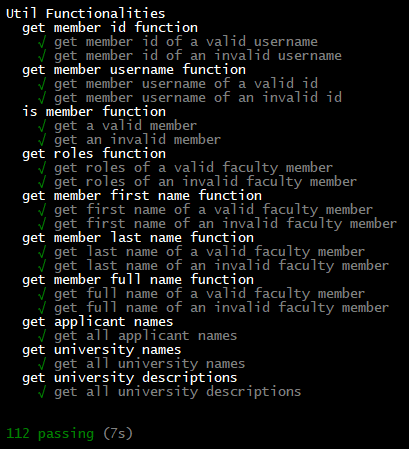
\includegraphics[width=.6\textwidth]{images/database/run_test.png}
\end{center}
\caption{Running Test}
\label{fig:db/run_test}
\end{figure} 

\newpage
\subsubsection{Test coverage}
Once the test suite has completed running it will give a resulted output of the code coverage from the database test suite. The code coverage is also saved in the source directory under ``coverage" folder.

\bigskip
\noindent Example of the code coverage output after running the database test suite:

\begin{figure}[!htb]
\begin{center}
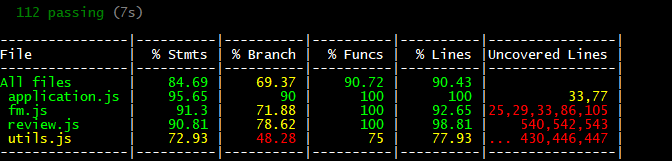
\includegraphics[width=.99\textwidth]{images/database/coverage.png}
\end{center}
\caption{Database Suite Coverage}
\label{fig:db/coverage}
\end{figure}

\newpage
\subsection{Application Tests}
The application test suite consists of a combination of acceptance tests with respect to the software requirement documentation and unit tests with respect to the software implementation. This suite is much more stronger than just an acceptance test suite as it covers more paths than an acceptance test suite would. The framework used for application tests is \textbf{Protractor}. To change the current directory to the application tests directory, do the following from the source directory:\\

\begin{lstlisting}[language=bash]
  $ cd test\specs\unit
\end{lstlisting}

\bigskip
\noindent Following is an example of an application test case:\\

\begin{lstlisting}
it('- log in with invalid password', function() {
	login.enterUsername(config.credentials.app.admin.username)
		.then(login.enterPassword.call(login, config.credentials.app.admin
			.password + '1'))
		.then(login.clickLogIn.call(login))
		.then(expect(browser.getCurrentUrl()).to.eventually
			.contain('login'))
		.then(expect(login.getErrorMessage.call(login)).to.eventually
		.equal('Invalid password. Please try again.'));
});
\end{lstlisting}

\newpage
\subsubsection{Add new test file}
Test files are separated by feature types. For example: review test, application test and faculty member test. To create a test file, do the following from the application suite directory:

\begin{lstlisting}[language=bash]
  $ touch <new_test_file>
\end{lstlisting}

\bigskip
\noindent Once a new test file has been creating, you can go ahead and start writing test cases. Following is an example test file with some test cases:\\

\begin{lstlisting}
describe('Login Test', function() {
	this.timeout(20000);

	var login = new Login();
	var role = new Role();
	var utils = new Utils();
	var welcome = new Welcome();

	before(function () {
		utils.startApp();
		utils.openView('#');
		utils.maximizeBrowserWindow();
		welcome.clickSignInButton();
	});

	after(function (done) {
		require('../../pretest');
		browser.restart();
		utils.stopApp(done);
	});

	it('- log in with only username no password', function() {
		login.enterUsername(config.credentials.app.admin.username)
			.then(login.clickLogIn.call(login))
			.then(expect(browser.getCurrentUrl()).to.eventually
				.contain('login'));
	});
    
	it('- log in with only password no username', function() {
		login.enterPassword(config.credentials.app.admin.password)
			.then(login.clickLogIn.call(login))
			.then(expect(browser.getCurrentUrl()).to.eventually
				.contain('login'));
	});
});
\end{lstlisting}

\newpage
\subsubsection{Running test suite}
Once you have added a new test file with some test cases you can simply run the entire application test suite using the following command from the source directory:

\begin{lstlisting}[language=bash]
	$ npm run unit:test
\end{lstlisting}

\bigskip
\noindent \textbf{Pro-tip}: 
\begin{itemize}
\item To run a single test file or a single test case , add \emph{.only} to the \emph{describe} or \emph{it} hook respectively.
\item To skip a single test file or a single test case , add \emph{.skip} to the \emph{describe} or \emph{it} hook respectively.  
\end{itemize}

\bigskip
\noindent Example of a running test suite:

\begin{figure}[!htb]
\begin{center}
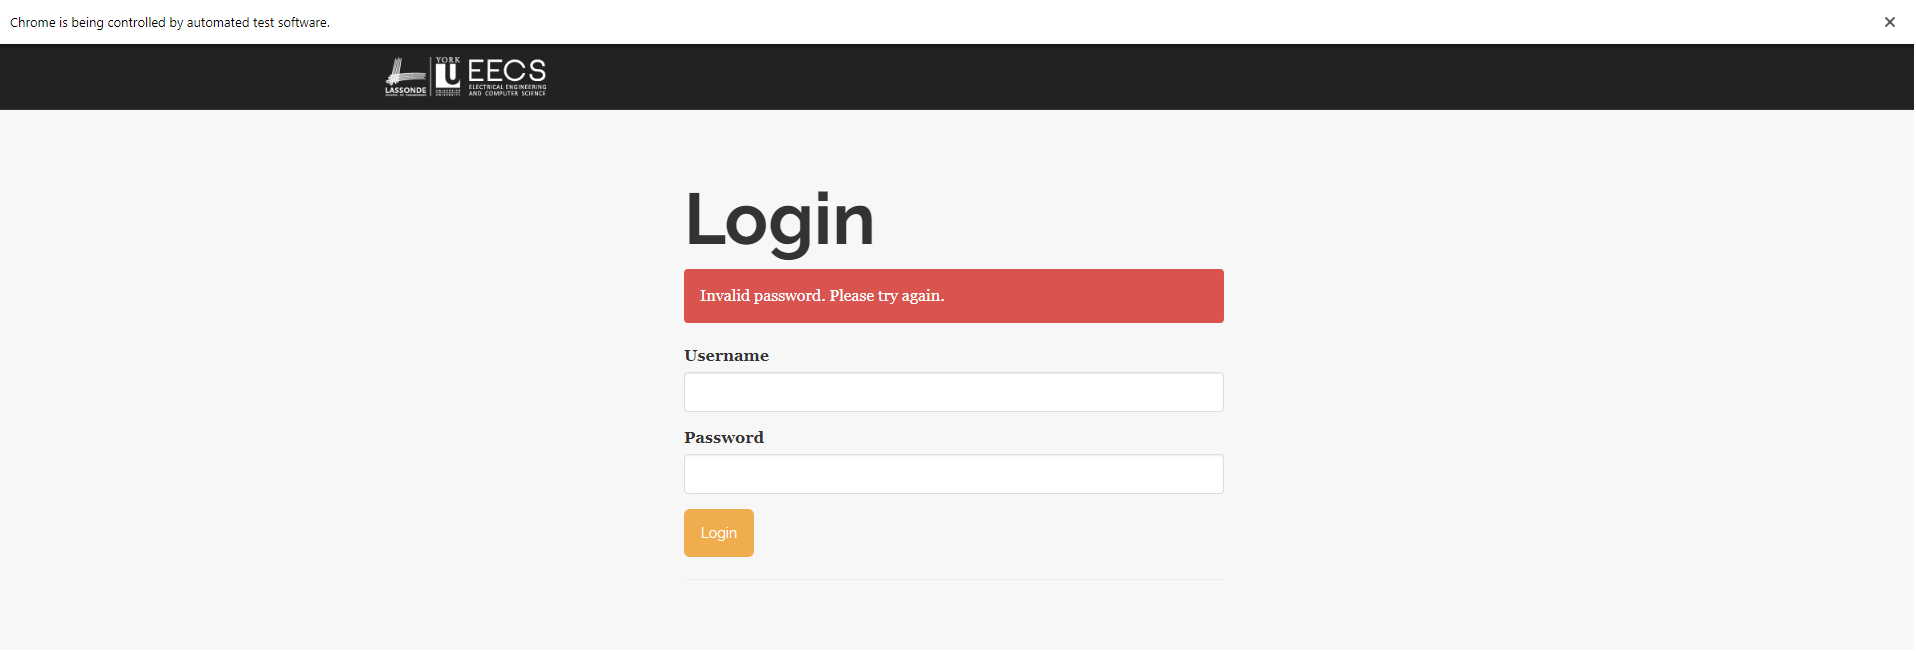
\includegraphics[width=.9\textwidth]{images/application/run_test.png}
\end{center}
\label{fig:app/run_test}
\end{figure}

\begin{figure}[!htb]
\begin{center}
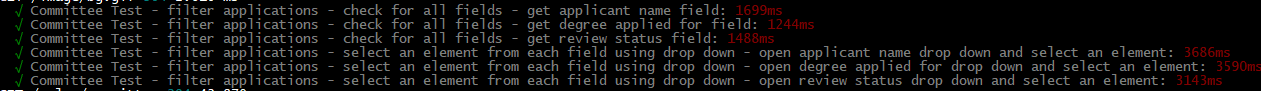
\includegraphics[width=.9\textwidth]{images/application/run_test2.png}
\end{center}
\caption{Running Test}
\label{fig:app/run_test2}
\end{figure}

\newpage
\subsubsection{Test coverage}
Once the test suite has completed running it will give a resulted output of the code coverage from the database test suite. The code coverage is also saved in the source directory under ``coverage" folder.

\bigskip
\noindent Example of the code coverage output after running the application test suite:

\begin{figure}[!htb]
\begin{center}
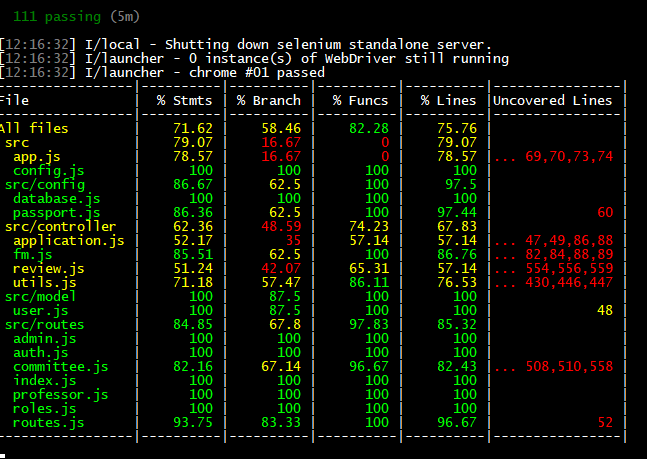
\includegraphics[width=.9\textwidth]{images/application/coverage.png}
\end{center}
\label{fig:app/coverage}
\end{figure}


\newpage
\subsection{Overall Tests}
The overall test suite consists of running both the database and application test suites.

\subsubsection{Running test suite}
To run the overall test suite use the following command from the source directory:

\begin{lstlisting}[language=bash]
	$ npm test
\end{lstlisting}

\bigskip
\noindent \textbf{Pro-tip}: 
\begin{itemize}
\item To run a single test file or a single test case , add \emph{.only} to the \emph{describe} or \emph{it} hook respectively.
\item To skip a single test file or a single test case , add \emph{.skip} to the \emph{describe} or \emph{it} hook respectively.  
\end{itemize}

\bigskip
\noindent Example of running the overall test suite:

\begin{figure}[!htb]
\begin{center}
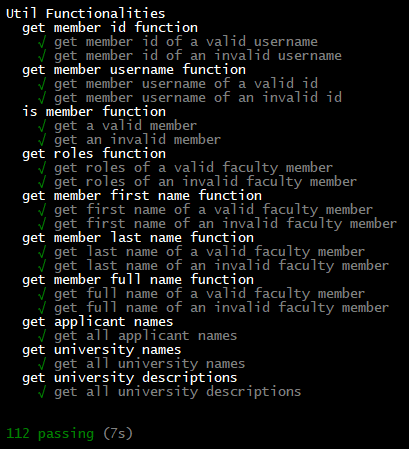
\includegraphics[width=.6\textwidth]{images/database/run_test.png}
\end{center}
\label{fig:db/run_test}
\end{figure} 

\begin{figure}[!htb]
\begin{center}
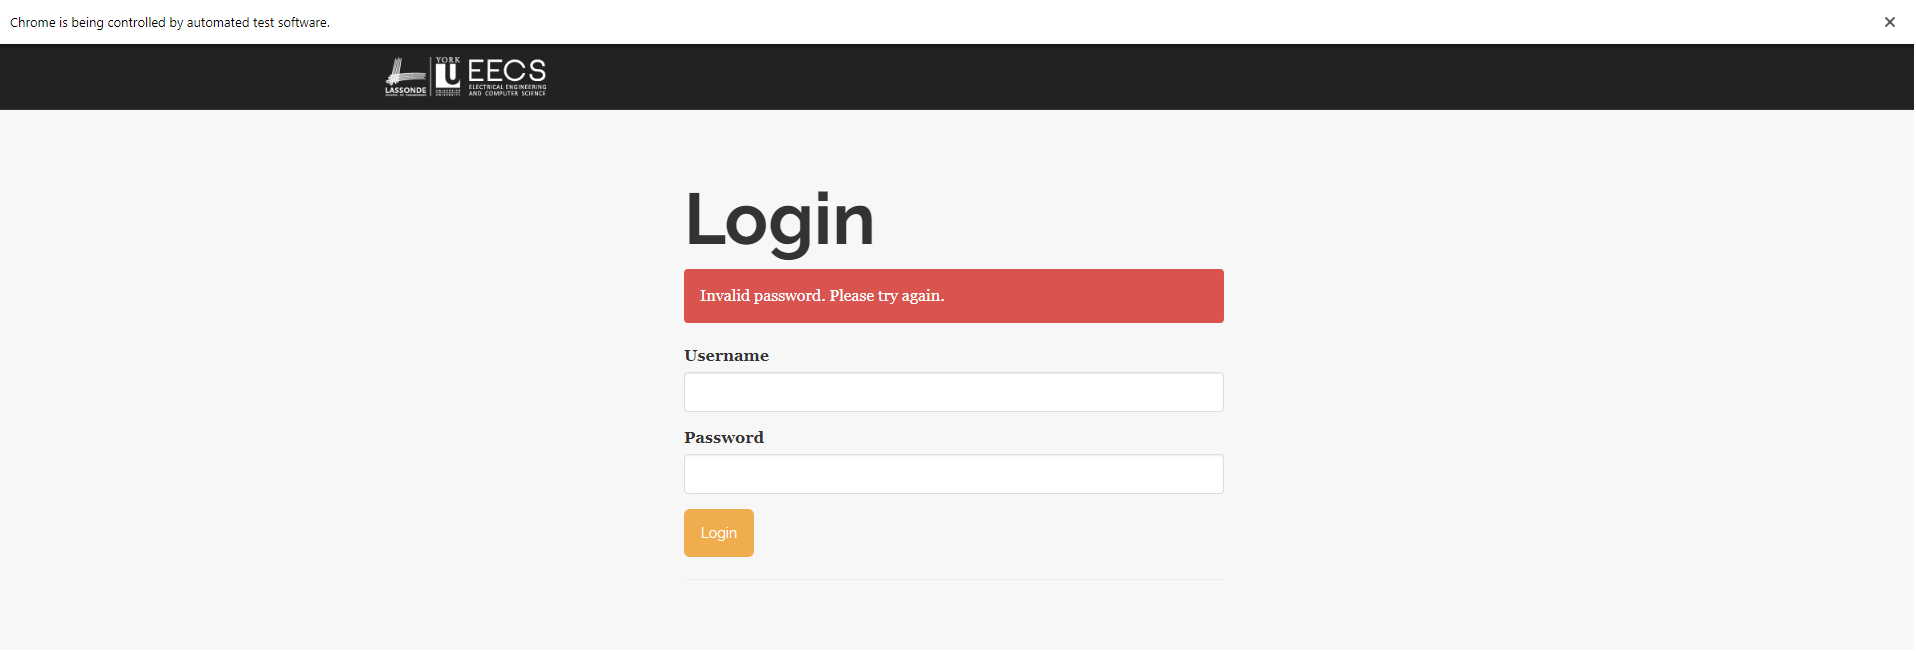
\includegraphics[width=.9\textwidth]{images/application/run_test.png}
\end{center}
\label{fig:app/run_test}
\end{figure}

\begin{figure}[!htb]
\begin{center}
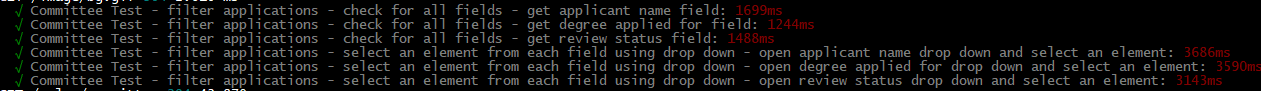
\includegraphics[width=.9\textwidth]{images/application/run_test2.png}
\end{center}
\caption{Running Overall Test Suite}
\label{fig:app/run_test2}
\end{figure}

\newpage
\subsubsection{Test coverage}
Once the test suite has completed running it will give a resulted output of the code coverage from the database test suite. The code coverage is also saved in the source directory under ``coverage" folder.

\bigskip
\noindent Example of the code coverage output after running the overall test suite:

\begin{figure}[!htb]
\begin{center}
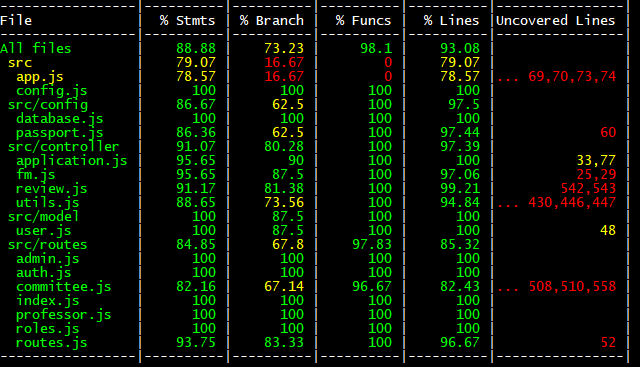
\includegraphics[width=.9\textwidth]{images/coverage.png}
\end{center}
\label{fig:overall/coverage}
\end{figure}

\newpage
\section{SQL Injection}
SQL injection is a code injection technique that may corrupt the underlying database of an application. It is one of the most common web hacking techniques in the world today. It works by simply placing malicious code in SQL statements, via web page inputs.

\bigskip
\noindent Our test suite, both database and application, covers protection against SQL injection. The application code for \hl{each of the controllers} in our MVC model asserts the input to be of the specified type we are hoping for. Any unmatched types will throw an exception making such asserts a crucial part of the application code.

\bigskip
\noindent Injecting malicious SQL statements through the controller will result in throwing such exceptions. This is because the SQL call is built by escaping the user inputs in a safe manner after the input is verified. Since, it can never reach the stage of a malicious type input within the controller, our application is safe from SQL injection.

\section{Code Linter}
The final execution after running a test suite is to lint the code to fix any syntactic or formatting issues in the code. This is done automatically as part of the post test, however, if one wants to lint the code at any point, they can simply do so by running the following command from the source directory.


\begin{lstlisting}[language=bash]
	$ npm run lint
\end{lstlisting}

\section{Coverage and Sufficiency}
\begin{quote}
``Program testing can be used to show the presence of bugs, but never to show their absence!'' - Dijkstra.
\end{quote}

\noindent Testers live and breed \hl{trade-offs}. Coverage measurements is a good tool to show \emph{how far} you are from complete testing, but a lousy tool to be used for investigating how close you are to complete testing. The time needed for tests related tasks is infinitely larger than the time available. Hence, it is impossible to fully test a software system in a reasonable amount of time or money.

\bigskip
\noindent That being said for the purpose of this project we have chosen to meet a minimum requirement of 80\% code coverage. With that we are confident enough to release a usable application.
\end{document}